% id: 118-e2
% book: 개념원리 확률과 통계 · 12 확률변수와 확률분포
% section: 필수·발전 예제
% figure: crop:fig-118-e2.png
% answer: $\dfrac{7}{8}$
% answer_source: 본문 풀이
% variant_level: 0 (원본 전사)
% 이 파일은 build.mjs 가 items.json 에서 만든다. 고칠 때는 items.json 을 고친다.
\smash{\raisebox{1.5mm}{\dmkichul{개념원리 확률과 통계 118쪽 예제 2 · 필수}}}
확률변수 $X$의 확률분포가 다음 표와 같을 때, $\mathrm{P}(X\ge a)$를 구하시오. \cond{$a$는 상수이다.}
\par\smallskip\begin{center}\setlength{\dmfigw}{193.9pt}\ifdim\dmfigw>\linewidth\setlength{\dmfigw}{\linewidth}\fi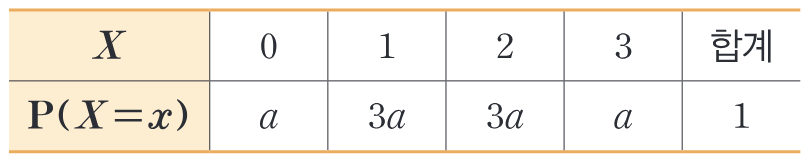
\includegraphics[width=\dmfigw]{figures/fig-118-e2.png}\end{center}
